
\documentclass[twocolumn]{article}
\usepackage{mathpazo}
\usepackage{microtype}
\usepackage{times}
\usepackage{titlesec} % 1
%\usepackage{sectsty} % "제 1 절" ...

 %%%%%%%%%%%%%%%%%%%%%%%%%%%%%%%%%%%%%%%%%%%%%%%%%%%%%%%%%%%%%%%%%%%%%%%%%%%%%
 %                              My Commands
\newcommand{\bi}{\begin{itemize}}
\newcommand{\ei}{\end{itemize}}
\newcommand{\be}{\begin{enumerate}}
\newcommand{\ee}{\end{enumerate}}
\newcommand{\ii}{\item}
\newtheorem{Def}{Definition}
\newtheorem{Lem}{Lemma}
\usepackage{algorithm}
\usepackage{algorithmicx}
\usepackage{algpseudocode}

\usepackage{graphicx}
\graphicspath{%
        {converted_graphics/}
        {./images/}
}

\usepackage[hangul,nonfrench,finemath]{kotex}
%\usepackage{kotex}    

\setlength\textwidth{7in} 
\setlength\textheight{9.5in} 
\setlength\oddsidemargin{-0.25in} 
\setlength\topmargin{-0.25in} 
\setlength\headheight{0in} 
\setlength\headsep{0in} 
\setlength\columnsep{9pt}
\sloppy 
 
\begin{document}

\title{
\vspace{-0.5in}\rule{\textwidth}{2pt}
\begin{tabular}{ll}\begin{minipage}{4.75in}\vspace{6px}
\noindent\large {\it KIWI Project}@Data Management Research Section\\
\vspace{-12px}\\
\noindent\LARGE ETRI\qquad  \large Technical Report 14ZS1410-TR-64
\end{minipage}&\begin{minipage}{2in}\vspace{6px}\small
218 Gajeong-ro, Yuseong-gu\\
Daejeon, 305-700, South Korea\\
http:/$\!$/www.etri.re.kr/\\
http:/$\!$/sungsoo.github.com/\quad 
\end{minipage}\end{tabular}
\rule{\textwidth}{2pt}\vspace{0.25in}
\LARGE \bf 다중 저장소 지속성 \\
\large Polyglot Persistence
}

\date{}

\author{
{\bf Sung-Soo Kim}\\
\it{sungsoo@etri.re.kr}
}

\maketitle

\begin{abstract}
{\small
본 기술문서에서는 RDBMS와 NoSQL 데이터 저장소와 같은 다양한 데이터 소스를 수용하여 고객의 요구사항에 따라 민첩하게 대응할 수 있는 방법인 다중 저장소 지속성(polyglot persistence)에 대해 기술한다. 다중 저장소 지속성이란 다양한 데이터 저장소 요건에 대해 다른 데이터 저장소 기술을 사용하는 것이다.

다중 저장소 지속성은 엔터프라이즈 환경이나 단일 애플리케이션에 적용할 수 있다. 또한, 데이터 접근을 서비스로 캡슐화하면 시스템의 각 부분에서 다른 데이터 저장소를 사용하더라도 영향을 최소화할 수 있다는 장점을 제공한다. 하지만, 데이터 저장소 기술을 추가할수록 프로그래밍과 운영 복잡도가 증가하므로, 데이터 저장소 도입의 장점과 복잡도 증가 문제의 경중을 따져봐야 한다.

}
\end{abstract}

\section{Introduction}

%\begin{figure}[!t]
%        \centering
%        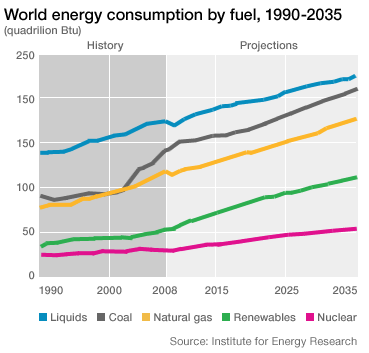
\includegraphics[width=0.33\textwidth]{test}
%        \caption{Caption}
%        \label{fig1}
%\end{figure}

 각 데이터베이스는 다른 문제를 풀 수 있도록 설계되었다. 모든 요구사항에 대해 하나의 데이터베이스 엔진을 사용해 만든 솔루션은 성능 기준을 충족하지 못할 수 있다. 트랜잭션 데이터 저장, 세션 정보 캐싱, 고객과 고객의 친구가 구입한 제품의 그래프 순회는 본질적으로 다른 문제다\cite{FOWLER:2013}. RDBMS 분야조차 OLAP(online analytical processing)과 OLTP(online transaction processing) 시스템의 요구사항은 매우 다르다. 그렇긴 하지만 같은 스키마에 틀어박는 경우도 가끔 있다. 

데이터 관계를 생각해 보자. RDBMS 솔루션은 이미 존재하는 관계를 강제할 때 좋지만, 관계를 새로 발견하고 싶거나 같은 객체에 속하는 데이터를 다른 테이블에서 찾아야 할 경우에는 사용하기 어려워진다.

데이터베이스 엔진은 여러 집합의 데이터나 한 저장소에서 동작하면서 키와 그 값을 매우 빠르게 읽거나 복잡한 문서나 그래프 정보를 저장하는 연산들과 같이 특정 구조와 특정 분량의 데이터에서 특정 연산을 아주 잘 처리하도록 설계되었다.

\section{Disparate Data Storage Needs}
많은 기업에서 비즈니스 트랜잭션, 세션 관리 데이터를 저장하는 데, 그리고 이와 다른 종류의 저장소를 필요로 하는 리포팅, BI, 데이터 웨어하우징, 로깅에 같은 데이터베이스 엔진을 사용하는 경향이 있다 (그림 \ref{fig01}).

\begin{figure}[!t]
        \centering
        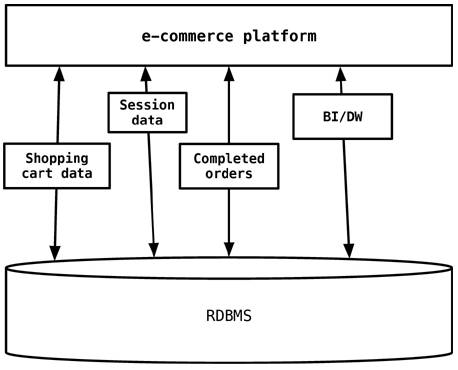
\includegraphics[width=0.42\textwidth]{rdbms}
        \caption{모든 데이터를 RDBMS에 저장}
        \label{fig01}
\end{figure}

세션, 장바구니 데이터에 대한 가용성과 일관성, 백업 요건의 수준은 주문 데이터에 필요한 수준과 같아야 할까? 세션 관리 저장소도 전자상거래 주문 데이터와 같은 엄격한 백업/복구 전략이 필요할까? 세션 관리 저장소가 세션 데이터를 읽고 쓰는 데 하나의 데이터베이스 인스턴스를 사용하는 것보다 높은 가용성이 필요할까?

2006년 닐 포드(Neal Ford)는, 문제마다 이를 해결하는 데 유리한 언어가 있으므로 이를 활용하기 위해 어플리케이션을 여러 언어로 작성해야 한다는 생각을 표현하려고 \textbf{다중 언어 프로그래밍(polyglot programming)}이란 용어를 만들었다. 복잡한 애플리케이션에는 여러 행태의 문제가 얽혀 있기 때문에, 한 언어로 모든 문제를 해결하기보다는 각 문제에 맞는 언어를 사용하는 것이 더 생산적이다.

전자상거래 시스템에서도 마찬가지다. 장바구니 데이터를 저장할 데이터베이스는 고가용성과 확장성이 중요하다. 그러나 고객의 친구들이 구입한 제품을 찾는 것은 완전히 다른 문제이므로 장바구니와 동일한 데이터 저장소를 사용하는 것은 도움이 되지 않는다. 여러 종류의 저장소를 사용하는 방법을 정의하기 위해 여기서는 \textbf{다중 저장소 지속성}이란 용어를 사용한다.

\section{Polyglot Data Store Usage}
전자상거래 예제에서 다중 저장소 지속성을 어떤식으로 적용할 수 있는지 살펴보자(그림 \ref{fig02}).
고객이 주문을 확정하기 전 장바구니 데이터와 세션 데이터는 키-밸류 저장소(key-value store)에 저장할 수 있다.
따라서 RDBMS에는 이런 일시적 데이터를 저장하지 않게 된다. 장바구니는 보통 사용자 아이디로 접근하고, 사용자 주문을 확정하여 결제하면 그때 RDBMS에 저장할 수 있으므로 여기에 키-밸류 저장소를 사용하는 것은 충분히 타당하다. 세션 데이터 역시 세션 아이디를 키로 사용할 수 있으므로 마찬가지다.

\begin{figure}[!t]
        \centering
        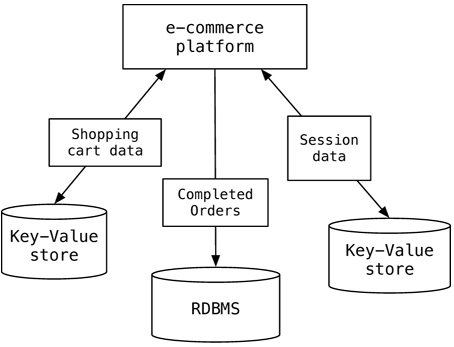
\includegraphics[width=0.42\textwidth]{session}
        \caption{세션 데이터와 장바구니 데이터를 키-밸류 저장소에 저장}
        \label{fig02}
\end{figure}

고객이 장바구니에 상품을 추가할 때 "당신의 친구들은 이런 제품도 구입했습니다." 또는 "당신의 친구들은 이 제품의 이런 액세서리도 함께 구입했습니다." 같이 상품을 추천하는 것이 필요하다면 그래프 데이터 저장소를 도입하는 것이 타당하다 (그림 \ref{fig03}).

\begin{figure}[!t]
        \centering
        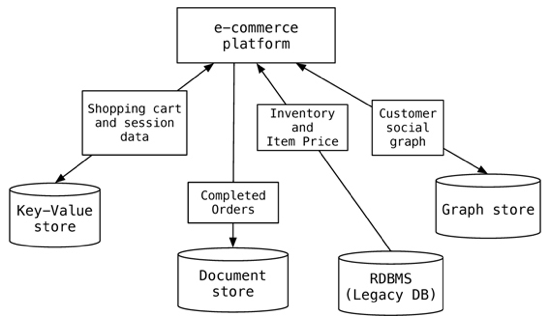
\includegraphics[width=0.42\textwidth]{graphstore}
        \caption{다중 저장소 지속성 구현 예}
        \label{fig03}
\end{figure}

각 데이터베이스는 다른 목적으로 구축되었고, 모든 문제를 한 데이터베이스로 우아하게 풀 수 있는 것도 아니므로, 애플리케이션에서도 모든 경우에 대해 한 가지 데이터 저장소를 고집할 필요는 없다.

한 애플리케이션에서 데이터 웨어하우스 어플라이언스나 분석 어플라이언스 같은 특화된 관계형 데이터베이스를 사용하는 것도 다중 저장소 지속성으로 볼 수 있다.

\section{Service Usage over Direct Data Store Usage}
애플리케이션에서 여러 종류의 데이터 저장소를 사용하도록 했을 때, 다른 애플리케이션에서 이쪽 데이터 저장소를 사용하거나 데이터를 이용할 필요가 있을 수 있다. 앞에서 사용한 전자상거래 예제에서, 그래프 데이터 저장소가 다른 애플리케이션, 예를 들면 특정 부류의 고객이 어떤 제품을 구입했는지 알아야 하는 애플리케이션에 데이터를 제공할 수 있다.

\begin{figure}[htb]
        \centering
        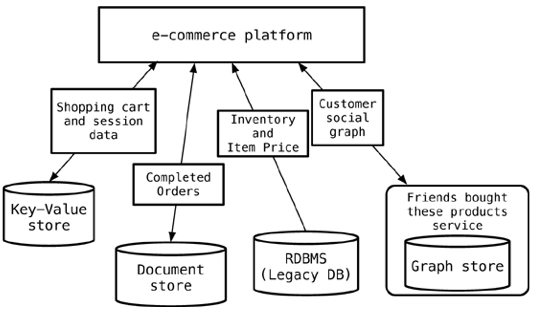
\includegraphics[width=0.42\textwidth]{warpping}
        \caption{데이터 저장소를 서비스로 감싼 구현 예}
        \label{fig04}
\end{figure}

그래프 데이터베이스에 각 애플리케이션이 독립적으로 접근하게 하는 대신, 그래프 데이터베이스를 서비스로 감싸서 모든 애플리케이션이 노드 사이의 관계를 한 장소에 저장하고 조회하게 할 수 있다(그림 \ref{fig04}).
한 애플리케이션이 여러 데이터베이스와 통신하게 하는 것보다는 서비스를 통해 데이터와 API를 제공하는 것이 더 유용하다.

서비스로 감싸는 방식을 좀 더 밀어붙여, 모든 데이터베이스를 서비스로 감싸 애플리케이션이 서비스하고만 통신하도록 할 수 있다(그림 \ref{fig05}). 이렇게 하면 종속된 애플리케이션을 변경하지 않고도 서비스 안에 데이터베이스를 변경할 수 있다.

\begin{figure}[htb]
        \centering
        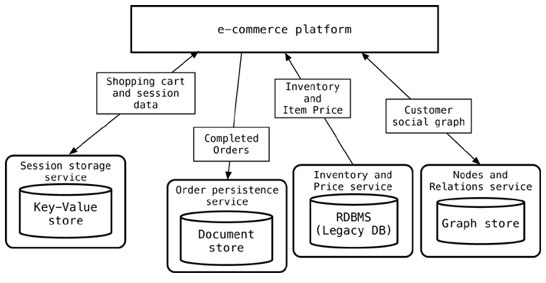
\includegraphics[width=0.42\textwidth]{services}
        \caption{데이터베이스와 통신하는 대신 서비스를 사용}
        \label{fig05}
\end{figure}

실제로 리아[Riak], 네오[Neo4J] 같은 많은 NoSQL 데이터 저장소 제품이 REST API를 제공한다.

\section{Expanding for Better Functionality}
기존 레거시 애플리케이션 및 기존 데이터 저장소와의 종속성 때문에 데이터 저장소를 변경하지 못하는 경우가 많다. 그러나 캐시를 추가해 성능을 개선하거나 솔라[Solr] 같은 색인 엔진을 사용해 검색 효율을 높이는 것처럼 기능을 추가할 수는 있다(그림 \ref{fig06}). 이런 기술을 도입할 때 애플리케이션이 사용하는 데이터 저장소와 캐시 또는 색인 엔진의 데이터가 동기화되도록 해야 한다.

\begin{figure}[htb]
        \centering
        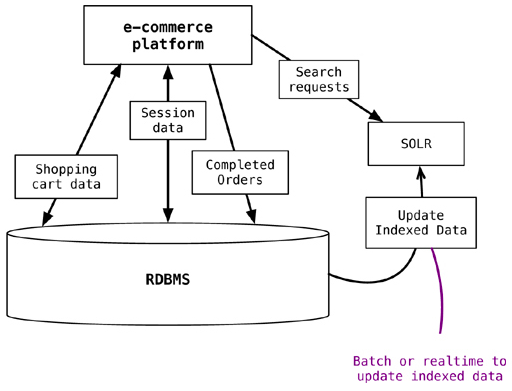
\includegraphics[width=0.42\textwidth]{storage}
        \caption{레거시 저장소 개선을 위한 추가 보조 저장소 사용}
        \label{fig06}
\end{figure}

애플리케이션이 사용하는 데이터베이스의 데이터가 변경될 때 색인 데이터도 업데이트해야 한다. 데이터는 실시간으로 업데이트할 수도 있고, 색인/검색 엔진에 있는 데이터가 최신이 아니어도 애플리케이션에 큰 영향이 없는 경우에는 배치 작업으로 일괄 업데이트할 수 있다. 색인을 업데이트하는 데는 이벤트 소싱 패턴을 사용할 수 있다.

이벤트 소싱(event sourcing)은 애플리케이션의 현재 상태만 저장하는 것이 아니라 상태의 모든 변화를 포착해 저장하는 것이다. 이벤트 소싱은 구조 패턴으로 관계형 데이터베이스를 포함한 대부분의 지속성 기술에서 잘 동작한다. 여기서 이벤트 소싱을 언급하는 이유는 이벤트 소싱이 지속성에 대한 특이한 사고방식에 근거를 제공하기 때문이다.

\section{Choosing the Right Technology}
다양한 데이터 저장소 솔루션이 있다. 처음에는 추세가 전문 데이터베이스에서 RDBMS 데이터베이스로 이동했다. 관계형 데이터베이스에는 추상화가 약간 필요하지만 모든 형태의 데이터 모델을 저장할 수 있다. 이제 추세는 애플리케이션 데이터를 그대로 저장할 수 있는 데이터 저장소를 사용하는 쪽으로 돌아오고 있다.

장바구니에 있는 제품을 기반으로 비슷한 제품을 구매한 고객이 다른 어떤 제품을 구매했는지 확인해 이를 추천하고 싶은 경우, 이 질문에 답할 수 있도록 적절한 속성과 데이터를 저장하면 어떤 데이터 저장소를 사용하든 구현할 수 있다. 여기서, 요령은 알맞은 기술을 이용하는 것이다. 그래야 질문이 바뀌어도 같은 데이터 저장소에서 기존 데이터를 버리거나 새로운 형식으로 변경하지 않고 동작할 수 있을 것이다.

다시 상품 추천 문제로 돌아가보자. RDBMS에서도 테이블을 적절히 설계해 계층적 쿼리를 이용하면 이 문제를 풀 수 있다. 그러나 순회 방식 변경이 필요한 경우 데이터베이스를 리팩터링해 데이터를 전환해야 하고 새로운 형식으로 데이터를 저장해야 한다. 노드 사이의 관계를 추적할 수 있는 데이터 저장소를 사용한다면, 프로그램을 작성해 새로운 관계를 표현할 수 있게 해 데이터 저장소 변경을 최소화할 수 있다.

\section{Enterprise Concerns with Polyglot Persistence}
NoSQL 데이터 저장소 기술의 등장으로 기업의 DBA도 이 새로운 저장소 활용 방법을 고민하지 않을 수 없게 됐다. 기업에서는 한결같이 RDBMS 환경을 유지했다. 어떤 데이터베이스든 사용하기 시작하면 향후 수년간은 모든 애플리케이션이 같은 데이터베이스를 사용해 구축될 가능성이 크다. 다중 저장소 지속성의 새로운 세상에서 DBA 그룹은 여러 기술을 익혀야 한다. NoSQL 기술이 어떻게 동작하는지, 이런 시스템을 어떻게 모니터링하는지, 백업은 어떻게 하는지, 시스템에 데이터를 어떻게 넣고 빼는지 배워야 한다.

어떤 NoSQL 기술이든 기업에서 사용하기로 결정했다면 라이선스, 지원, 도구, 업그레이드, 드라이버, 감사, 보안 등의 사항이 문제로 떠오른다. 많은 NoSQL 기술이 오픈 소스고, 활동이 왕성한 지지자 커뮤니티가 있다. 상업적 지원을 제공하는 회사도 있다. 아직 도구 생태계는 풍부하지 않지만, 도구 제작사와 오픈 소스 커뮤니티가 따라잡고 있으며, 몽고DB 모니터링 서비스[Monitoring], 데이터스택스 오피에스 센터[Ops Center] 또는 리악을 위한 레콘브라우저[Rekon] 같은 도구를 발표하고 있다.

기업이 우려하는 다른 부분은 보안 문제다. 데이터베이스 수준에서 사용자를 생성하고 데이터를 볼 수 있거나 없도록 권한을 할당할 수 있는 기능이 여기에 포함된다. NoSQL 데이터베이스는 대부분 견고한 보안 기능을 갖추기 못했지만, 이는 NoSQL이 다른게 동작하도록 설계되었기 때문이다. 전통적인 RDBMS에서는 데이터베이스가 데이터를 직접 제공하고 쿼리 도구가 있긴 하지만 기본 사상은 다르다. NoSQL에서는 애플리케이션이 데이터를 소유하고 서비스를 사용해 데이터를 제공한다. 이런 방식에서는 보안에 대한 책임이 애플리케이션에 있다. 그렇지만, 보안 기능을 도입한 NoSQL 기술도 있긴 하다.

기업에는 흔히 다중 데이터 저장소에 있는 데이터를 필요로 하는 데이터 웨어하우스 시스템, BI, 분석 시스템이 있다. 따라서, ETL (extract-transform-load) 도구가 지원되는지, 소스 시스템에서 데이터 웨어하우스로 데이터를 옮기는 데 현재 사용하고 있는 도구가 NoSQL 데이터 저장소에 있는 데이터를 읽을 수 있는지 확인해야 한다. 여러 ETL 도구 제작사가 NoSQL과 통신할 수 있는 도구를 출시하고 있다. 예를 들어, 펜타호[Pentaho]는 몽고DB와 카산드라 데이터를 읽을 수 있다.

모든 기업은 어떤 형태든 분석을 실행한다. 포착해야 하는 데이터 크기가 급증함에 따라, 이 모든 데이터를 데이터베이스에 저장하도록 RDBMS 시스템을 확장하려고 많은 기업이 고투하고 있다. 엄청난 빈도의 쓰기와 쓰기 확장성이 필요한 경우에는 NoSQL 데이터베이스가 잘 맞는다. NoSQL을 사용하면 엄청난 양의 데이터를 기록할 수 있다.

\section{Deployment Complexity}
일단 애플리케이션에서 다중 저장소 지속성을 사용하기로 했다면, 배포 복잡성에 대해 주의 깊은 고민이 필요하다. 이제 실 환경에서 모든 데이터베이스가 동시에 필요하다. 개발 환경, QA 환경, 검수 테스트 환경에도 모든 데이터베이스가 필요하다. NoSQL 제품은 대부분 오픈 소스기 때문에, 라이선스 비용 문제는 거의 없다. 자동 설치, 설정도 지원된다. 예를 들어, 데이터베이스를 설치하려면 다운로드해 압축을 풀면 그만인데, curl과 unzip 명령을 이용해 자동화 할 수 있다. 이런 NoSQL 제품은 적절한 기본 설정이 되어 있으며, 최소한의 설정 변경으로 시작할 수 있다.

\section{Key Points}

\begin{itemize}
  \item 다중 저장소 지속성이란 다양한 데이터 저장소 요건에 대해 다른 데이터 저장소 기술을 사용하는 것이다.
  \item 다중 저장소 지속성은 엔터프라이즈 환경이나 단일 애플리케이션에 적용할 수 있다.
  \item 데이터 접근을 서비스로 캡슐화하면 시스템의 각 부분에서 다른 데이터 저장소를 사용하더라도 영향을 최소화할 수 있다.
  \item 데이터 저장소 기술을 추가할수록 프로그래밍과 운영 복잡도가 증가하므로, 데이터 저장소 도입의 장점과 복잡도 증가 문제의 경중을 따져봐야 한다.
\end{itemize}

\bibliographystyle{IEEEtran}
\bibliography{References}























































\end{document}
